\chapter{Preliminary analysis of \ac{AABW} samples}
\label{ch:deepappendix}

\section{Summary}

TODO write this

\section{Introduction and Methods}
\begin{table}
\caption[\ac{AABW} samples used in the preliminary analysis]{Sampling time, location and physicochemical properties of \ac{AABW} samples used in this preliminary study.
All data were retrieved from the \ac{CTD} (SeaBird, Bellevue, USA) instrument used to collect the samples.}
\label{tab:deepsamples}
\smallskip
\begin{tabularx}{\textwidth}{llllXXXXXX}
\toprule
\textbf{Sample} & \textbf{Date} & \textbf{Latitude} & \textbf{Longitude} & \textbf{Sample Depth (m)} & \textbf{Temperature (\textdegree{}C)} & \textbf{Salinity (PSU)} & \textbf{Volume \linebreak filtered (L)}\\
\midrule

356 & 03/01/08 & $-66.7617$ & 144.4138 & 920 & $-1.9$ & 34.69 & 230\\
361 & 14/01/08 & $-66.4727$ & 140.5572 & 1170 & $-1.8$ & 34.56 & 225\\
365 & 23/01/08 & $-56.6967$ & 141.9125 & 3693 & 0.5 & 34.69 & 230\\
\bottomrule
\end{tabularx}
\end{table}

% the sample map
\begin{figure}
  \centering
  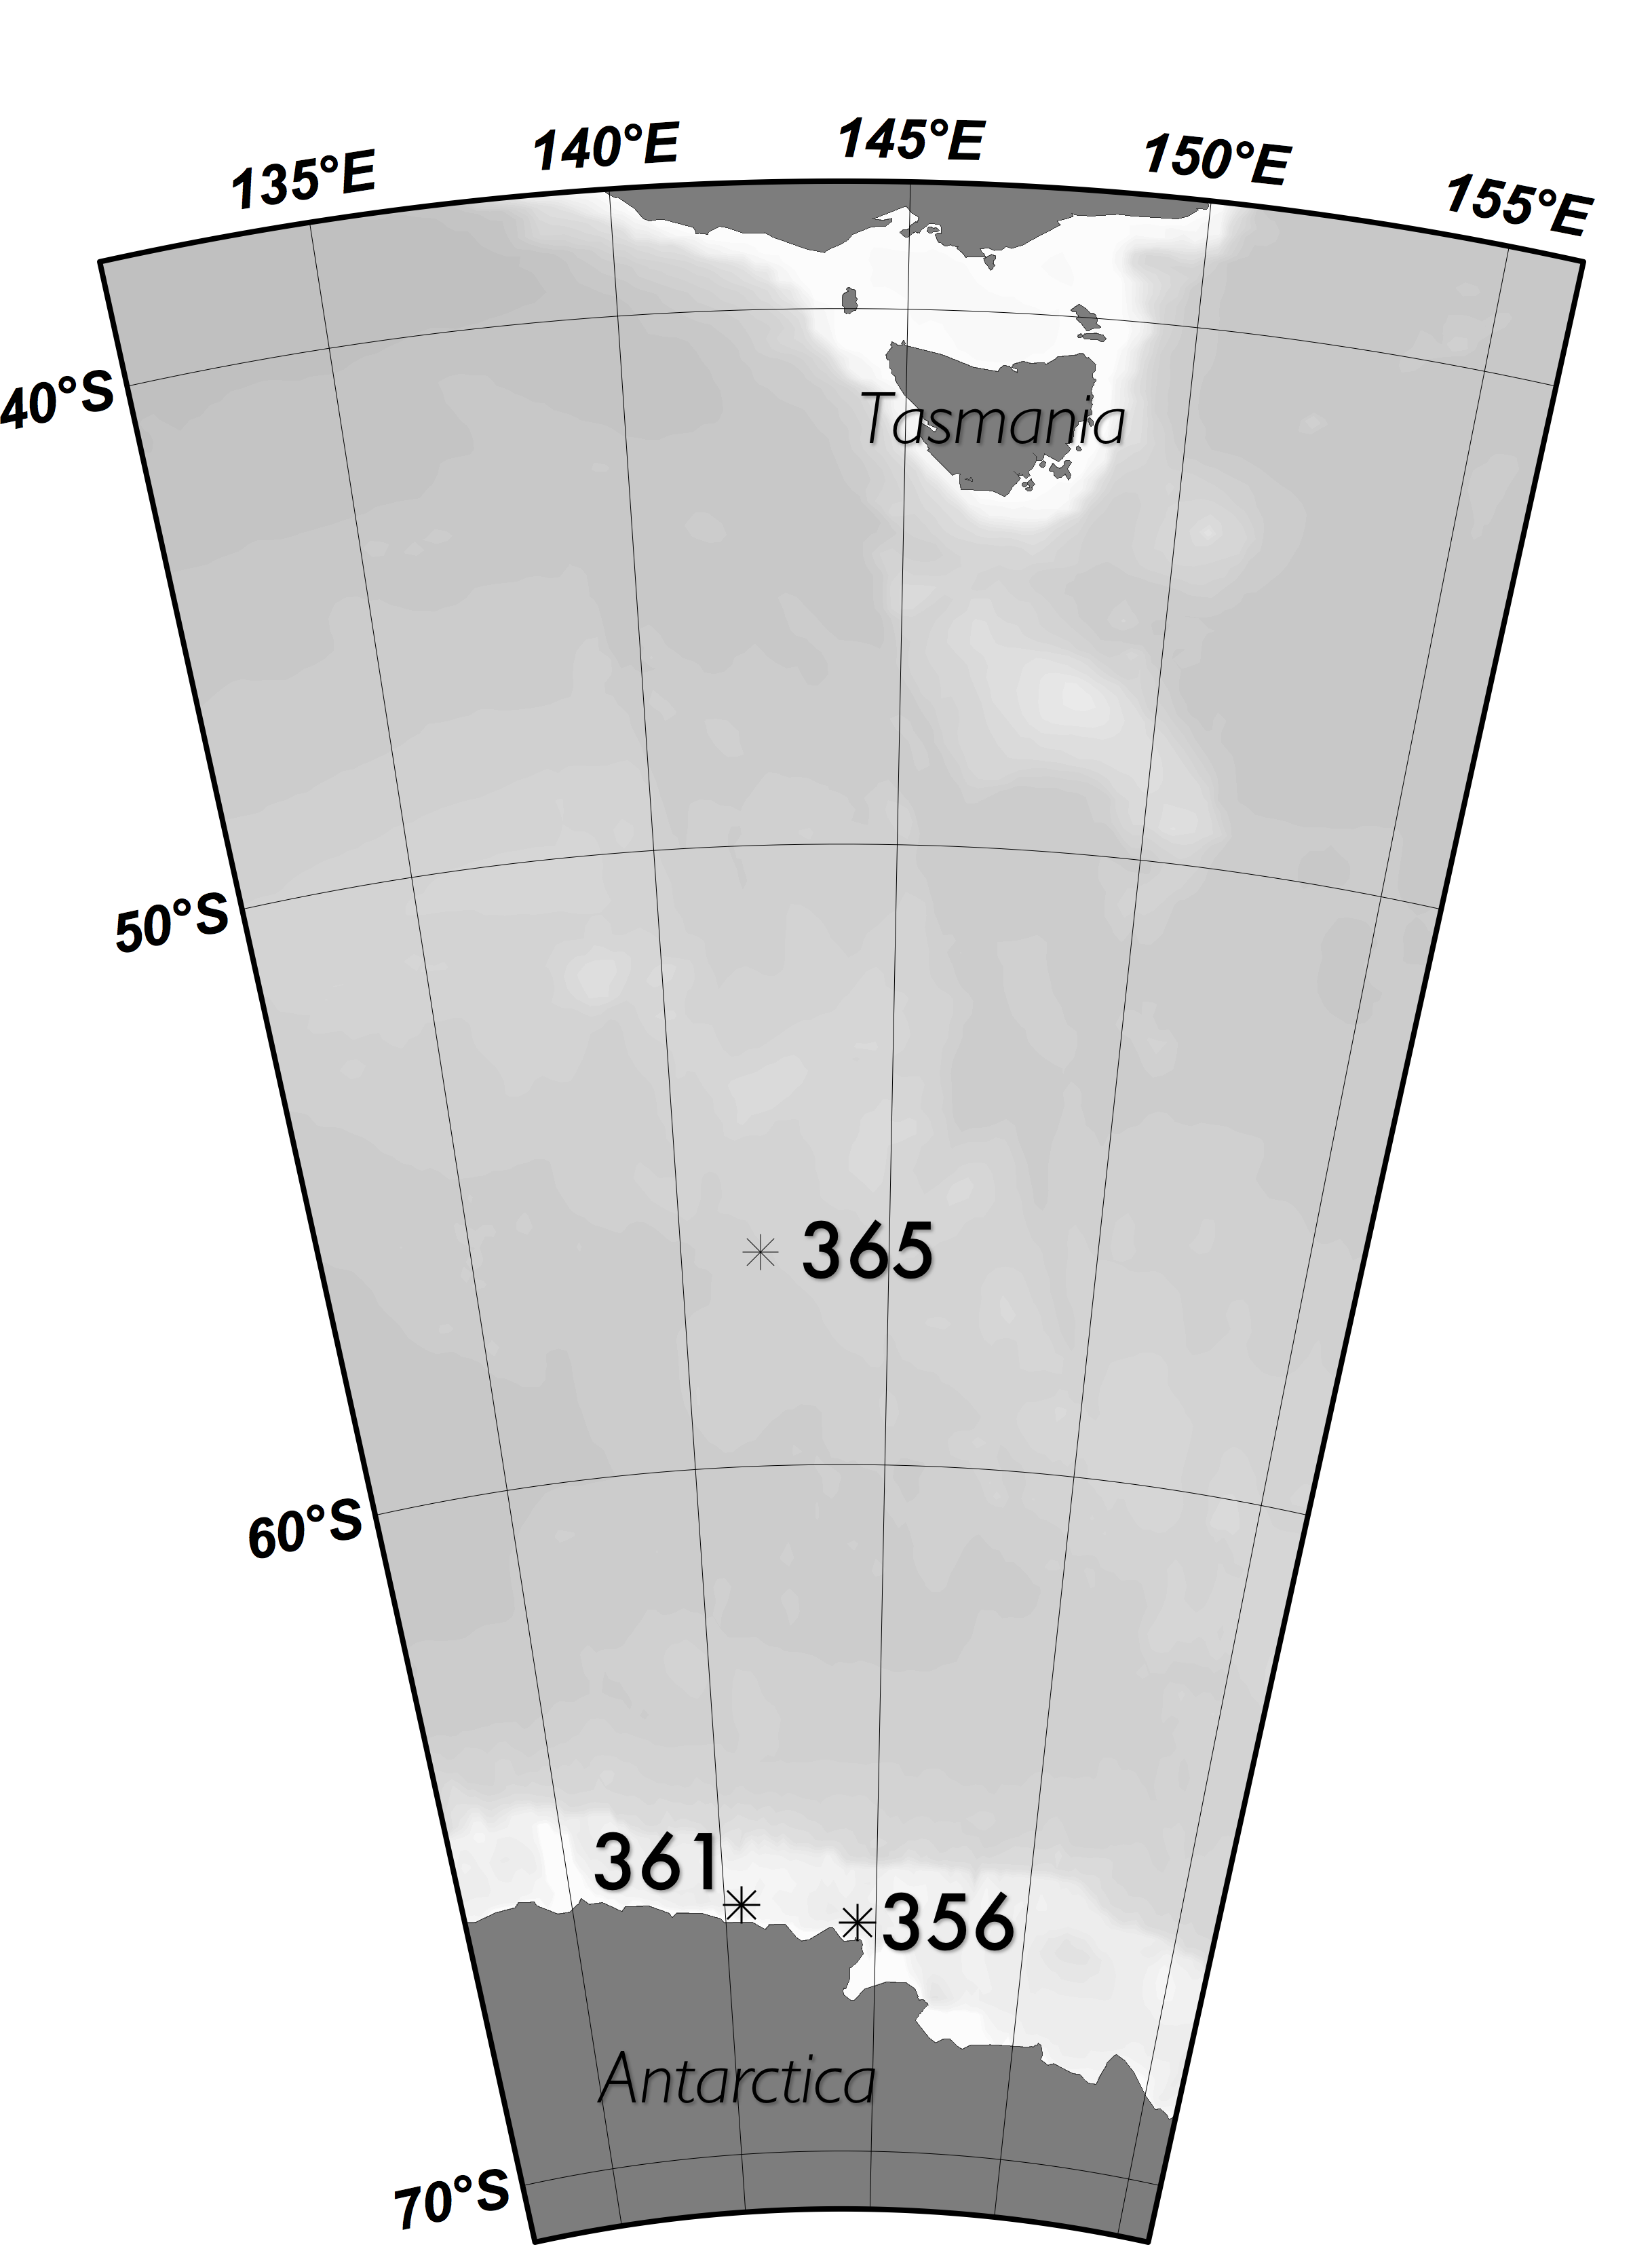
\includegraphics[width=\textwidth]{../advection/deepsamplemap.png}
  \caption[Map showing sites of preliminary \ac{AABW} samples]{Sites of preliminary \ac{AABW} samples.}
  \label{fig:deepsamplemap}
\end{figure}

Three samples of \ac{AABW} were opportunistically obtained and analysed during the project described in \secreft{ch:polarfront} \figref{fig:deepsamplemap}.
Two of these samples (356 and 361) were of newly formed \ac{AABW} waters on the Antarctic continental shelf, while one (365) was of abyssal \ac{AABW} from the South Australian basin \tabref{tab:deepsamples}.
DNA extraction, sequencing and construction of a taxonomic profile by \softwarename{blast} comparison to the RefSeq database and processing with \ac{GAAS} were performed using the methods described in \secreft{ch:polarfront}.
A standardised and log-transformed Bray-Curtis resemblance matrix was constructed including the taxonomic profiles of the \ac{AABW} samples as well as the \ac{NZ} and \ac{SZ} samples described in \secreft{ch:polarfront}.
A \ac{nMDS} plot was then constructed from this matrix.
All statistical procedures were performed in \softwarename{PRIMER 6} as described by \citet{Clarke:2001ut}.

\section{Results and Discussion}

Although the three \ac{AABW} samples were taken in deep, cold and aphotic waters \tabref{tab:deepsamples} compared to the surface \ac{AZ} and \ac{SZ} samples, the \ac{nMDS} plot suggested that the two continental shelf \ac{AABW} samples (356 and 361) were surprisingly similar to those of the \ac{AZ}, particularly sample 353 \figref{fig:deepnmds}.
Further, the indicated the presence of several \acp{OTU} which would not be expected to be present at significant abundance in deep, aphotic waters \tabref{tab:topdeepotus}.
For example, \species{Roseobacter denitrificans} OCh 114, a model organism for aerobic anoxygenic photosynthesis, was the fifth most abundant \ac{OTU} across the three \ac{AABW} samples.
Numerous \ac{CFB} representatives, typically associated with \ac{POM} and the utilisation of \ac{HMW} phytoplankton products, were also unexpectedly high.

\begin{table}
\footnotesize
\caption[Twenty most abundant \acp{OTU} in preliminary \ac{AABW} samples]{Relative abundances (as percentages) of the twenty most abundant \acp{OTU} identified in the preliminary study of \ac{AABW} samples.}
\label{tab:topdeepotus}
\smallskip
\begin{tabularx}{\textwidth}{Xllllll}
\toprule
\textbf{OTU} & \multicolumn{3}{c}{\textbf{Sample 356}} & \multicolumn{3}{c}{\textbf{Sample 365}}\\
\cmidrule(r){2-4}
\cmidrule(r){5-7}
& 0.1 \micron & 0.8 \micron & 3.0 \micron & 0.1 \micron & 0.8 \micron & 3.0 \micron\\
\midrule
\candidatusfull{Pelagibacter ubique} HTCC1062 & 48.40 & 32.32 & 32.85 & 19.02 & 22.31 & 3.880\\
\speciesfull{Nitrosopumilus maritimus} SCM1 & 11.92 & 9.289 & 13.99 & 30.17 & 7.790 & 22.74\\
\candidatusfull{Ruthia magnifica} str. Cm (\species{Calyptogena magnifica}) & 3.780 & 4.563 & 2.356 & 2.844 & 1.504 & 0.2599\\
\candidatusfull{Vesicomyosocius okutanii} strain HA & 2.349 & 2.757 & 1.396 & 1.859 & 0.8025 & 0.08227\\
\genus{Roseobacter} sp. OCh 114 & 0.1412 & 1.166 & 0.6845 & 0.08564 & 0.6662 & 0.4851\\
\candidatusfull{Puniceispirillum marinum} IMCC1322 & 0.3180 & 1.103 & 0.6403 & 0.4218 & 0.8223 & 0.4202\\
\species{Marinobacter hydrocarbonoclasticus} VT8 & 0.06999 & 0.4091 & 0.3976 & 0.2476 & 1.050 & 2.338\\
\species{Silicibacter pomeroyi} DSS-3 & 0.1081 & 0.8406 & 0.4996 & 0.1290 & 0.4630 & 0.3621\\
\species{Robiginitalea biformata} strain HTCC2501 & 0.2813 & 0.6433 & 0.7417 & 0.1769 & 0.2739 & 0.4978\\
\species{Pseudoalteromonas haloplanktis} strain TAC125 & 0.02530 & 0.4540 & 0.1958 & 0.2836 & 2.817 & 0\\
\species{Alcanivorax borkumensis} strain SK2 & 0.09262 & 0.3163 & 0.4281 & 0.1049 & 0.5674 & 1.985\\
\species{Gramella forsetii} strain KT0803 & 0.3096 & 0.6465 & 0.7405 & 0.1254 & 0.2670 & 0\\
\genus{Colwellia} sp. 34H & 0.04289 & 0.4512 & 1.020 & 0.07200 & 0.4532 & 0.7727\\
\species{Flavobacterium psychrophilum} strain JIP02/86 & 0.2417 & 0.4722 & 0.6353 & 0.07943 & 0.1645 & 0.5072\\
\species{Pirellula staleyi} strain DSM 6068 & 0.003149 & 0.2477 & 0.3093 & 0.08767 & 1.401 & 0.7732\\
\genus{Jannaschia} sp. DFL-12 & 0.07995 & 0.6770 & 0.3841 & 0.03865 & 0.2030 & 0.1025\\
\species{Pseudoalteromonas atlantica} strain T6c & 0.02312 & 0.1653 & 0.1941 & 0.03856 & 0.3235 & 1.728\\
\species{Zunongwangia profunda} strain SM-A87 & 0.1830 & 0.3499 & 0.4826 & 0.1036 & 0.1362 & 0.3825\\
\genus{Silicibacter} sp. TM1040 & 0.09568 & 0.5448 & 0.3455 & 0.03477 & 0.2014 & 0.1740\\
\species{Capnocytophaga ochracea} strain DSM 7271 & 0.1251 & 0.2916 & 0.4491 & 0.03893 & 0.1542 & 0.5332\\
\bottomrule
\end{tabularx}
\end{table}


A possible explanation for these observations is that the continental shelf samples represent \ac{AABW} recently formed in the D'Urville sea, and the observed assemblage therefore represents advection rather than selection by environmental factors.
The project described in \secreft{ch:advection} was designed to test and explore this hypothesis.

\begin{figure}
  \centering
  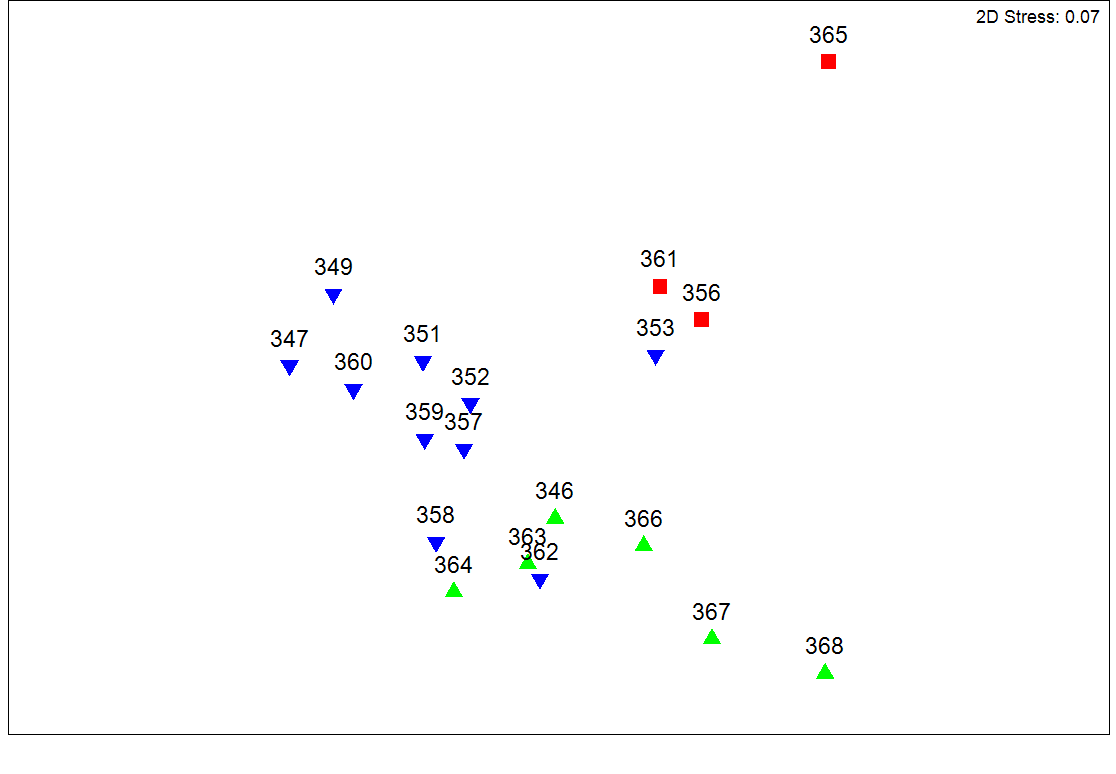
\includegraphics[width=\textwidth]{../advection/deepnmds.png}
  \caption[\ac{nMDS} of \ac{AABW}, \ac{NZ} and \ac{SZ} samples]{\ac{nMDS} plot showing distance between \ac{AABW}, \ac{NZ} and \ac{SZ} samples.
  Green triangles represent samples from the \ac{NZ}; blue inverted triangles from the \ac{SZ}; and red squares from \ac{AABW}.}
  \label{fig:deepnmds}
\end{figure}

